% FIG ch07-06 GLUT4 final overlay (English)
\definecolor{ch07comp}{HTML}{6B6B6B}
\definecolor{ch07transnote}{HTML}{C46A2A}
\definecolor{ch07act}{HTML}{3A3A3A}
\definecolor{ch07conv}{HTML}{7A7A7A}
\definecolor{ch07trans}{HTML}{E39B5B}
\definecolor{ch07flux}{HTML}{C46A2A}
\definecolor{ch07phos}{HTML}{E3B23C}
\begin{tikzpicture}
  \node[anchor=south west, inner sep=0] (img) at (0,0)
    {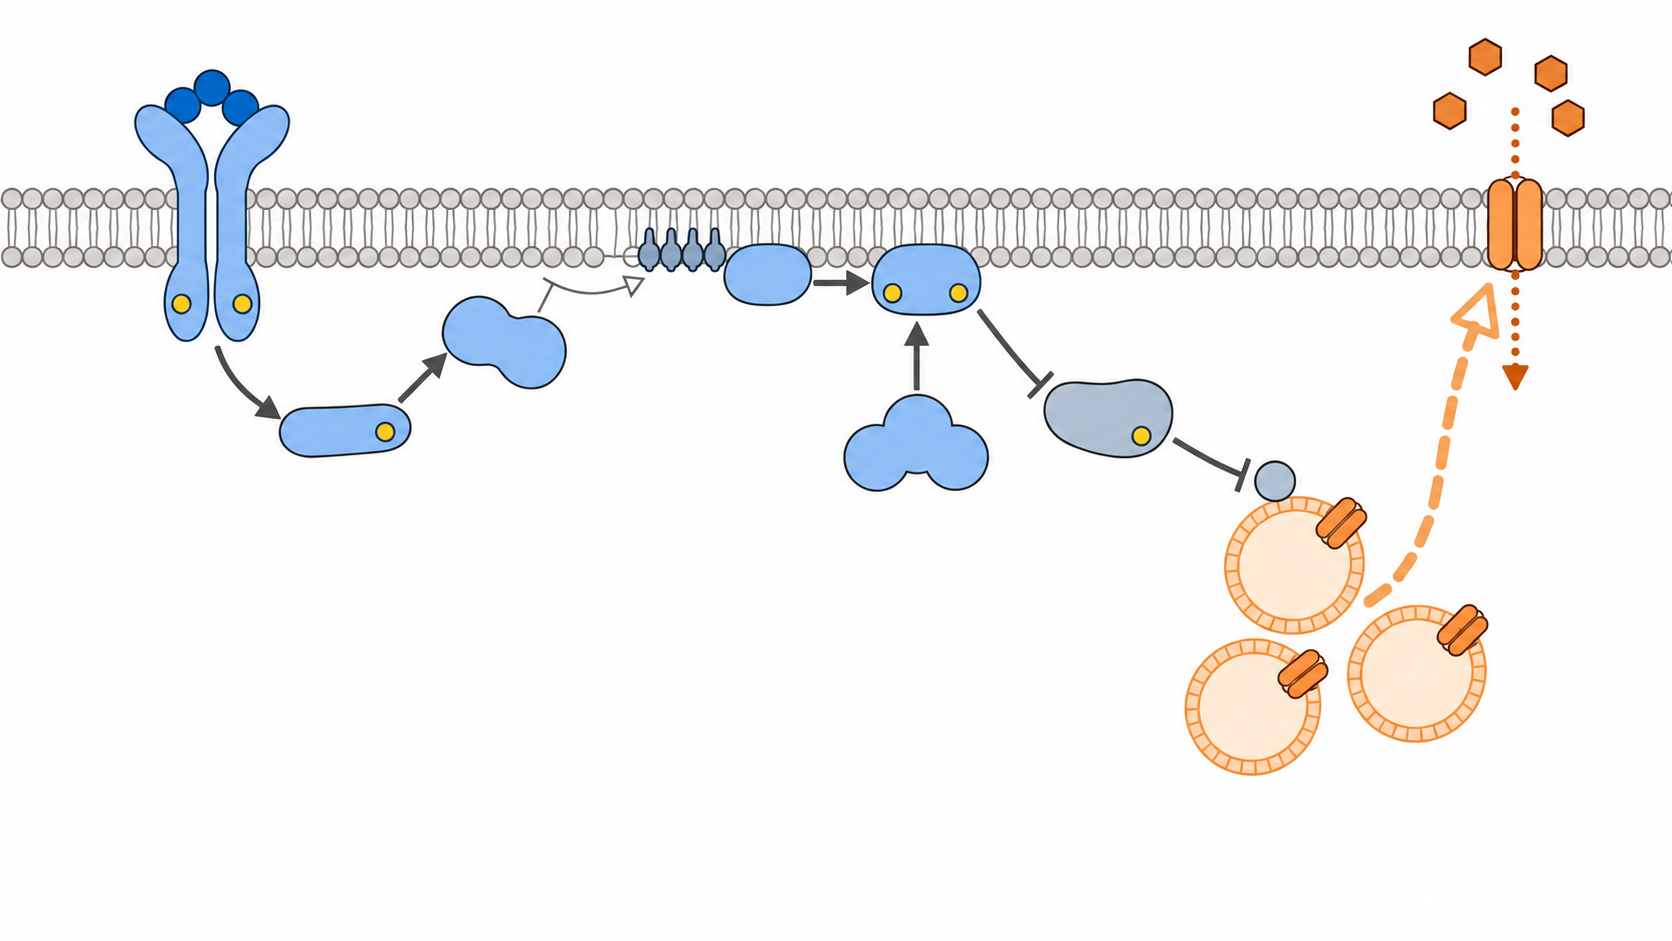
\includegraphics[width=\linewidth]{figures/ch07/ch07-06-v4-base.png}};
  \begin{scope}[x={(img.south east)}, y={(img.north west)},
    font=\sffamily\small]
    \node[text=ch07comp, font=\sffamily\footnotesize\itshape, anchor=west]
      at (0.04, 1-0.055) {Extracellular};
    \node[text=ch07comp, font=\sffamily\footnotesize\itshape]
      at (0.62, 1-0.15) {Plasma membrane};
    \node[text=ch07comp, font=\sffamily\footnotesize\itshape, anchor=west]
      at (0.04, 1-0.90) {Cytoplasm};
    \node[anchor=west, font=\sffamily\small] at (0.20, 1-0.06) {Insulin};
    \draw[BookInk!40, thin] (0.20, 1-0.065) -- (0.145, 1-0.10);
    \node[anchor=west, font=\sffamily\small] at (0.20, 1-0.145) {Insulin receptor};
    \draw[BookInk!40, thin] (0.20, 1-0.15) -- (0.16, 1-0.20);
    \node[font=\sffamily\small] at (0.21, 1-0.56) {IRS-1};
    \node[font=\sffamily\small] at (0.34, 1-0.50) {PI3K};
    \node[font=\sffamily\footnotesize] at (0.48, 1-0.075) {PIP\textsubscript{2} → PIP\textsubscript{3}};
    \draw[BookInk!40, thin] (0.44, 1-0.10) -- (0.385, 1-0.275);
    \node[font=\sffamily\small] at (0.46, 1-0.40) {PDK1};
    \node[font=\sffamily\small] at (0.515, 1-0.375) {Akt};
    \draw[BookInk!40, thin] (0.53, 1-0.36) -- (0.55, 1-0.335);
    \node[font=\sffamily\small] at (0.52, 1-0.60) {mTORC2};
    \draw[BookInk!40, thin] (0.54, 1-0.56) -- (0.55, 1-0.52);
    \node[align=center, font=\sffamily\footnotesize] at (0.80, 1-0.345) {AS160\\(TBC1D4)};
    \draw[BookInk!40, thin] (0.755, 1-0.385) -- (0.695, 1-0.42);
    % Two short lines in the white gap right of the Rab circle (x 0.78–0.84).
    \node[align=left, font=\sffamily\scriptsize, anchor=south west] at (0.788, 1-0.508) {Rab-\\GTP};
    \draw[BookInk!40, thin] (0.784, 1-0.500) -- (0.770, 1-0.512);
    \node[align=center, font=\sffamily\small, anchor=north] at (0.78, 1-0.85) {GLUT4 storage\\vesicles};
    \draw[BookInk!40, thin] (0.78, 1-0.845) -- (0.78, 1-0.80);
    \node[font=\sffamily\small, anchor=west] at (0.94, 1-0.345) {GLUT4};
    \draw[BookInk!40, thin] (0.94, 1-0.33) -- (0.915, 1-0.26);
    \node[font=\sffamily\small, anchor=east] at (0.845, 1-0.065) {Glucose};
    \draw[BookInk!40, thin] (0.845, 1-0.075) -- (0.875, 1-0.09);
    % Right-aligned beside the dashed arrow; the long line stays right of x=0.87.
    \node[text=ch07transnote, font=\sffamily\scriptsize\itshape, align=right, anchor=north east]
      at (0.998, 1-0.430) {translocation\\\& fusion};
    \draw[ch07transnote!55, thin] (0.878, 1-0.448) -- (0.858, 1-0.432);
  \end{scope}
  \node[anchor=north west, font=\sffamily\scriptsize, align=left] at (img.south west) {%
    \begin{tabular}{@{}l@{\quad}l@{}}
      \tikz{\draw[-{Stealth[length=1.5mm]}, ch07act, line width=0.6pt] (0,0) -- (0.22,0);} Activation &
      \tikz{\draw[-{Bar[width=4pt]}, ch07act, line width=0.6pt] (0,0) -- (0.22,0);} Inhibition \\
      \tikz{\draw[ch07conv, line width=0.4pt] (0,0) .. controls (0.08,0.04) .. (0.18,0);} Enz.\ conv. &
      \tikz{\draw[ch07trans, line width=1pt, dashed] (0,0) -- (0.18,0);} Translocation \\
      \tikz{\draw[ch07flux, line width=0.6pt, dotted, -{Stealth[length=1.2mm]}] (0,0) -- (0.18,0);} Glucose flux &
      \tikz{\fill[ch07phos] (0.09,0) circle (1.2pt);} Phosphorylation
    \end{tabular}};
\end{tikzpicture}
